\section{Experiment Results}
\label{sec:experiment}

\subsection{Image Specific Class Model Visualization}
\label{subsec:visualization}
Given an image $I$, a class label $k$ and the hidden neuron activation states $h$, we approximate the neural net class score $S_k$ with the first-order taylor expansion in the neighborhood of $I$:
\begin{equation}
  S_k(I, h) \approx  T_k(h)^T I + b
\end{equation}
where $T_k(h)$ is the derivative of $S_k$ with respect to the image at the point of $I$ and hidden neuron status $h$.

$T_k(h)$ can be also viewed as the linear template applied on image $I$ for the understanding of how like the image belongs to class $k$. We can visualize $T$ since it's the same size as the image $I$. We use this technique to visualize the model through the paper.

Specifically, for a VggNet~\cite{Simonyan2014Very} which uses only a stack of piece-wise linear layers (i.e.\ convolution, relu, max-pooling) to compute the class scores, once the hidden states $h$ encodes the selection of linear functions for each piece-wise linear operator, the final score is an linear operation on the image, equivalent to the inner product between the template and the image.

\textbf{Comparison of Methods:} We compare the visualization and saliency extraction of the feedbacked results against~\cite{simonyan2013deep} (Oxford) and~\cite{zeiler2014visualizing} (Deconv) on a set of complex images containing multiple objects from different classes. We show the qualititative results in Figure~\ref{fig:examples}. All techniques use the same pre-trained VggNet\cite{Simonyan2014Very} and ground truth class labels for each image are given. The visualization results before feedback is the same as Oxford, where all the hidden neurons states are determined by bottom-up computation. The visualization results after the feedback process are similar to Deconv, except that our model captures the most salient visual regions for each specific class. 

\textbf{Comparison of ConvNet Models:} We compare the three most popluar ConvNets: AlexNet~\cite{Krizhevsky2012ImageNet}, VggNet~\cite{Simonyan2014Very} and Googlenet~\cite{Szegedy2014Going} by visualizing their feedback templates in Figure~\ref{fig:model_compare}. All models are pre-trained on Caffe with the same classificatino accuracy reported. Ground truth class labels are given for each image before feedback. From the visualization results, we find that VggNet and GoogleNet produce more accurate visual attention than AlexNet, suggesting the benefit of using smaller convolution filters and deeper architectures to further distinguish similar and closeby objects. We also observe that, although both VggNet and GoogleNet produce very smilar image classification accuracies, GoogleNet better captures the salient object areas for each class than VggNet. We hypothesize that the two 4096 dimensional fully connected layers (i.e.\ fc6, fc7) in VggNet (which GoogleNet does not contain) could harm the spatial distinctiveness of the final image features,  

\textbf{Feedback Attention for Fine-Grained Classification:} We show some interesting feedback visualization results for understanding the fine-grained classifcation ability of VggNet~\cite{Simonyan2014Very}. The VggNet is trained on ImageNet dataset~\cite{deng2009imagenet} with 1000 object classes which contains $\sim$100 fine-graiend dog categories and $\sim$500 animal categories. We visualize the feedback templates of a few dog-cat images with respect to some dog classes and animal classes in Figure~\ref{fig:class_compare}. We observe that each object class has its own special salient image features for distinction. Given the fixed images, some classes tend to emphasize on local region features such as parts (i.e.\ nose and ears), while others focus on global attributes (i.e.\ furry and tabby).

\subsection{Weakly Supervised Object Localization}
\label{subsec:localization}
To quantitatively demonstrate the effectiveness of the feedback model. we experiment on the ImageNet 2014 localization task.

As pointed in~\cite{simonyan2013deep}, the magnitude of the elements in the model template $T_k$ in section~\ref{subsec:visualization} defines the class specific salience map for image $I$. A pixel with larger magnitude indicates that it is more important to the class $k$. We adopt the same saliency extraction strategy as~\cite{simonyan2013deep} that a single class saliency value $M_k$ for class $k$ at pixel $(i,j)$ is computed across all color channels: $M_k(i,j) = \max_{c \in rgb} | T_k(i,j,c) |$.

Although the ConvNet is pre-trained for image classification, we could use the feedbacked salience map for weakly supervised object localization. Following~\cite{simonyan2013deep}, given an image and the corresponding class saliency map, we compute the object segmentation mask using the GraphCut color segmentation~\cite{yuri2001interactive}. During the inialization of graph cut, We set the pixels with the saliency higher than 95\% quantile of the saliency distribution in the image as foreground and those with the saliency lower than 30\% quantile as background. Once foreground and background segmentations are computed, the object segmentation mask is set to the largest connected component of the foreground pixels and the tighest bounding box is extracted as the localization result.

We test our object localization method on the ImageNet 2014 localization validation set. We resize every image to 224x224 as the model required resolution and use the ground-truth class labels for the localization prediction. No further preprocessing or multi-scale strategy is involved. The predicted bounding box is considered as correct if its intersection over union with the ground truth bounding box is over 50\%. 

\textbf{Comparison of Methods:} Table~\ref{tab:localization_accuracy} shows the comparsion of weakly supervised localization accuracy against Oxford and Deconv. We use the same VggNet and apply the same graph cut strategy on all the 3 models. Our method obtains 57\% accuracy, outperforming both Oxford 50\% and Deconv 53\%, suggesting that in terms of capturing attention and localizing salient objects, our feedback net is better. Note that currently this is only top-down and weakly supervised and the object localization task is not taken into account during training.

\textbf{Comparsion of ConvNet Models:} We also compare the weakly supervised localization ability of the three most popular ConvNet models: AlexNet, VggNet and GoogleNet in Table~\ref{tab:localization_model_compare}, given the ground-truth class labels. AlexNet ... \textbf{\color{red} I need the number to complete the paragraph. } 

However, Most of the images in ImageNet 2014 dataset contain only one salient object. We further show some localization results on images with multiple object classes in Figure~\ref{} ... \textbf{\color{red} I need the figures to complete the paragraph}. Obviously our feedback net cannot distinguish multiple object instances from the same class, but could capture the salient areas, which could be utilized by other sophisticated object detection algorithms. 

\begin{table}
\centering
Localization Error With Top 5 Predictions
\begin{tabular}{|c|c|c|c|}
\hline
Method & AlexNet & VggNet & GoogleNet \\ 
\hline
Oxford~\cite{simonyan2013deep} & 53.4 & 51.6 & 47.8 \\
Deconv~\cite{zeiler2014visualizing} & 55.2 & 52.2 & 49.6\\
Feedback & 52.3 & 49.0 & \textbf{46.1} \\
\hline
\end{tabular}
\caption{We compare the localization results on ImageNet 2014 validation set against Oxford and Deconv, using three different ConvNet models. Our feedback method clearly outperforms the baseline approaches for weakly supervised object localization. Notably, although VggNet and GoogleNet have ery similar image classfication accuray on ImageNet, our comparison suggests GoogleNet learns better middle level features than VggNet.}
\label{tab:localization_accuracy_top5}
\end{table}

\begin{table}
\centering
Localization Error With Ground Truth Labels
\begin{tabular}{|c|c|}
\hline
Model & Localization Error (\%) \\ 
\hline
AlexNet~\cite{Krizhevsky2012ImageNet} & \\
VggNet~\cite{Simonyan2014Very} & 39.8 \\
GooglNet~\cite{Szegedy2014Going} & \\
\hline
\end{tabular}
\caption{In order to more fairly compare AlexNet agaisnt VggNet ana GoogleNet, we use the ground truth labels as the target labels for evaluating localization.}
\label{tab:localization_model_compare}
\end{table}

\begin{table}
\centering
Localization Error With Ground Truth Labels
\begin{tabular}{|c|c|}
\hline
Method & Localization Error (\%) \\
\hline
Oxford~\cite{simonyan2013deep} & 41.6 \\
Deconv~\cite{zeiler2014visualizing} & 42.5 \\
Feedback & \textbf{39.8} \\
\hline
\end{tabular}
\caption{We show that even given ground truth labels, our feedback method still outperforms baseline methods on ImageNet 2014 validation dataset.}
\label{tab:localization_accuracy}
\end{table}

\setlength{\tabcolsep}{2pt}
\begin{figure*}
\begin{center}
\begin{tabular}{c||ccc||ccc}
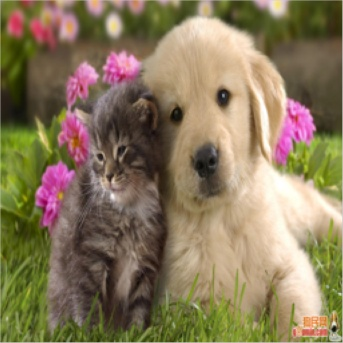
\includegraphics[width=0.13\linewidth]{figs/examples/googlenet/oxford/dog-cat1} &
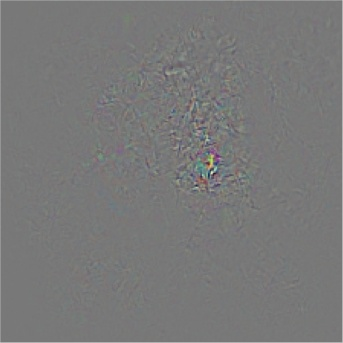
\includegraphics[width=0.13\linewidth]{figs/examples/googlenet/oxford/dog-cat1_diff_258} &
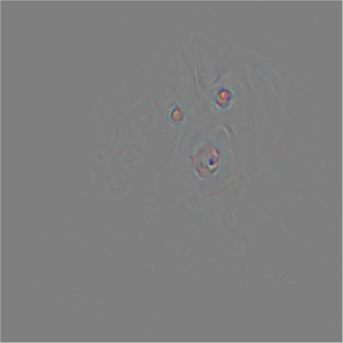
\includegraphics[width=0.13\linewidth]{figs/examples/googlenet/deconv/dog-cat1_diff_258} &
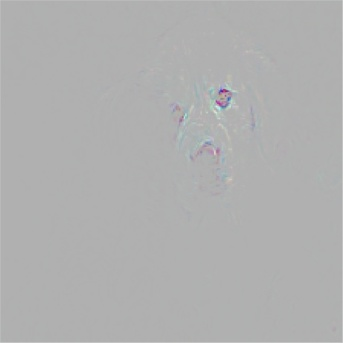
\includegraphics[width=0.13\linewidth]{figs/examples/googlenet/soft/dog-cat1_diff_258} &
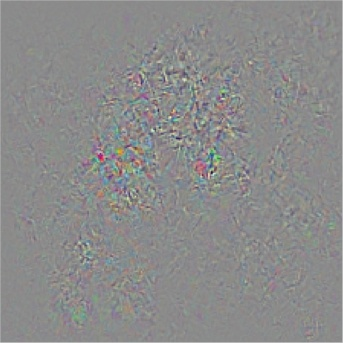
\includegraphics[width=0.13\linewidth]{figs/examples/googlenet/oxford/dog-cat1_diff_286} &
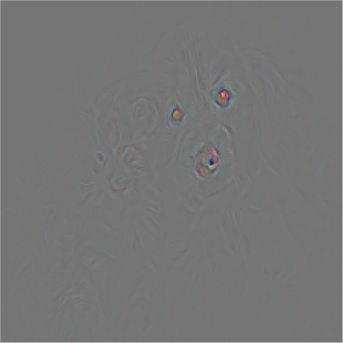
\includegraphics[width=0.13\linewidth]{figs/examples/googlenet/deconv/dog-cat1_diff_286} &
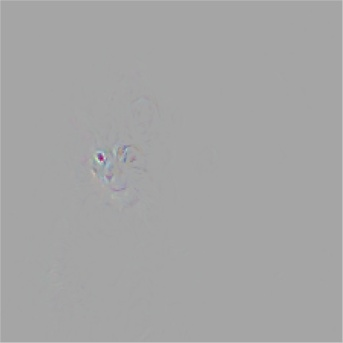
\includegraphics[width=0.13\linewidth]{figs/examples/googlenet/soft/dog-cat1_diff_286} \\
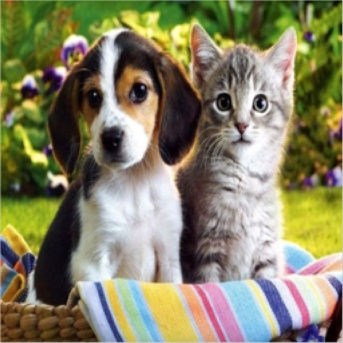
\includegraphics[width=0.13\linewidth]{figs/examples/googlenet/oxford/dog-cat2} &
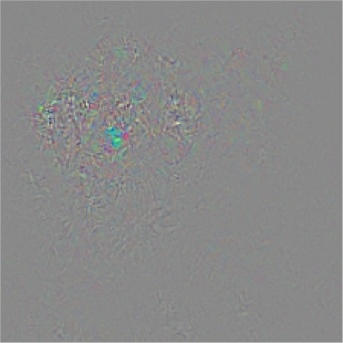
\includegraphics[width=0.13\linewidth]{figs/examples/googlenet/oxford/dog-cat2_diff_163} &
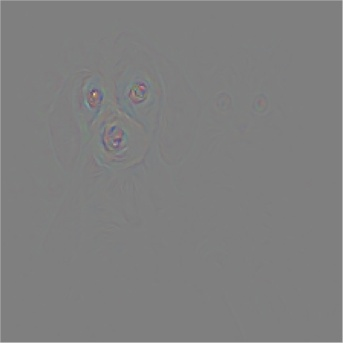
\includegraphics[width=0.13\linewidth]{figs/examples/googlenet/deconv/dog-cat2_diff_163} &
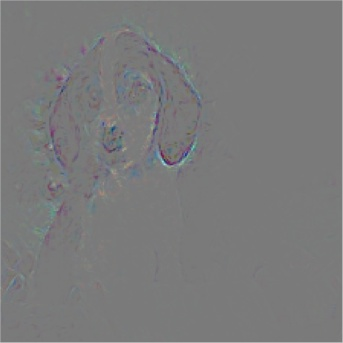
\includegraphics[width=0.13\linewidth]{figs/examples/googlenet/soft/dog-cat2_diff_163} &
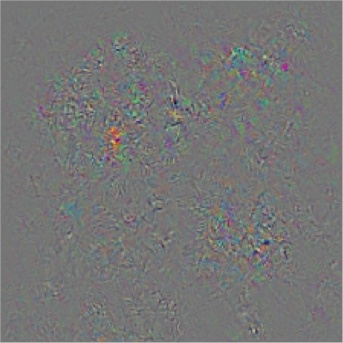
\includegraphics[width=0.13\linewidth]{figs/examples/googlenet/oxford/dog-cat2_diff_286} &
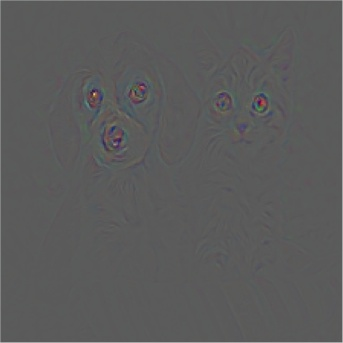
\includegraphics[width=0.13\linewidth]{figs/examples/googlenet/deconv/dog-cat2_diff_286} &
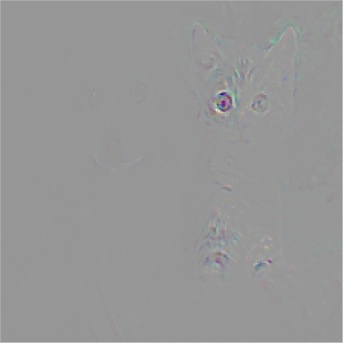
\includegraphics[width=0.13\linewidth]{figs/examples/googlenet/soft/dog-cat2_diff_286} \\
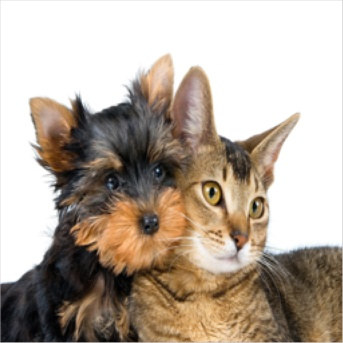
\includegraphics[width=0.13\linewidth]{figs/examples/googlenet/oxford/dog-cat3} &
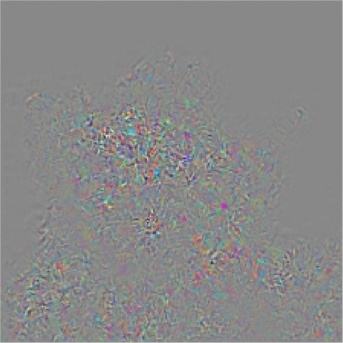
\includegraphics[width=0.13\linewidth]{figs/examples/googlenet/oxford/dog-cat3_diff_188} &
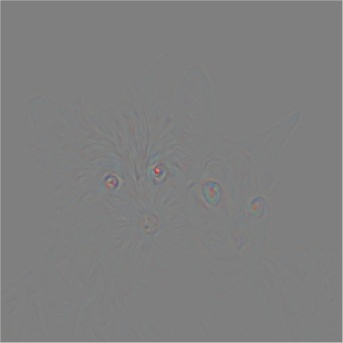
\includegraphics[width=0.13\linewidth]{figs/examples/googlenet/deconv/dog-cat3_diff_188} &
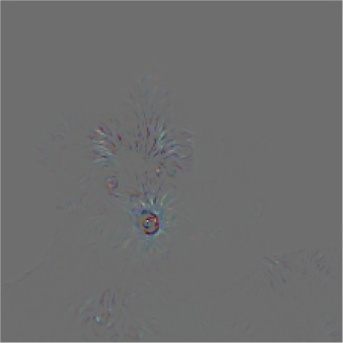
\includegraphics[width=0.13\linewidth]{figs/examples/googlenet/soft/dog-cat3_diff_188} &
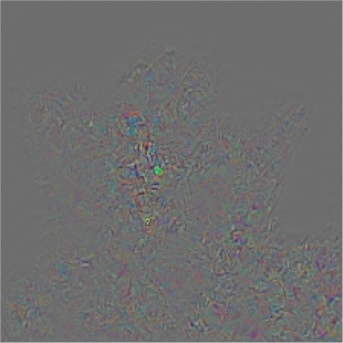
\includegraphics[width=0.13\linewidth]{figs/examples/googlenet/oxford/dog-cat3_diff_286} &
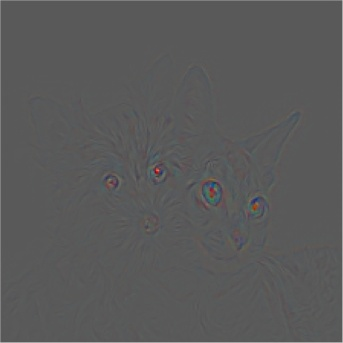
\includegraphics[width=0.13\linewidth]{figs/examples/googlenet/deconv/dog-cat3_diff_286} &
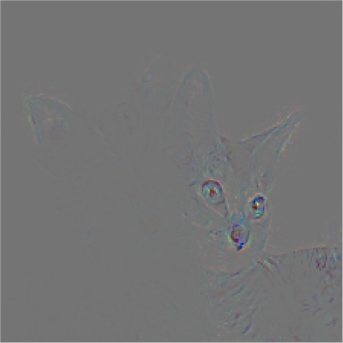
\includegraphics[width=0.13\linewidth]{figs/examples/googlenet/soft/dog-cat3_diff_286} \\
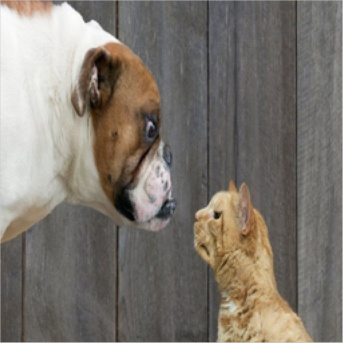
\includegraphics[width=0.13\linewidth]{figs/examples/googlenet/oxford/dog-cat4} &
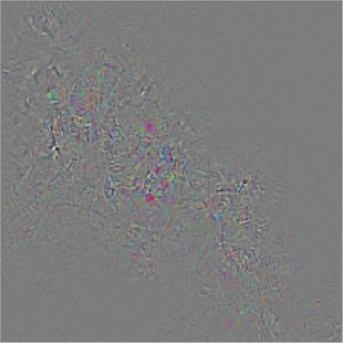
\includegraphics[width=0.13\linewidth]{figs/examples/googlenet/oxford/dog-cat4_diff_243} &
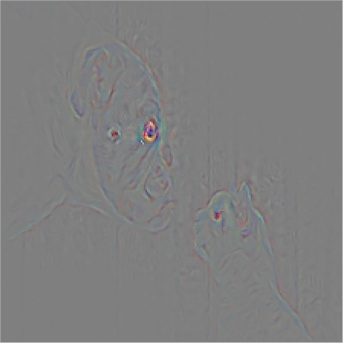
\includegraphics[width=0.13\linewidth]{figs/examples/googlenet/deconv/dog-cat4_diff_243} &
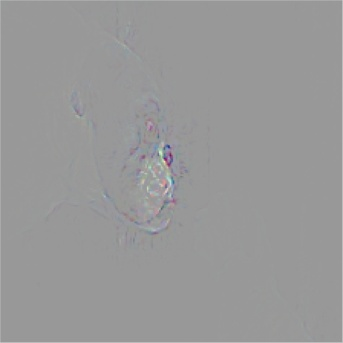
\includegraphics[width=0.13\linewidth]{figs/examples/googlenet/soft/dog-cat4_diff_243} &
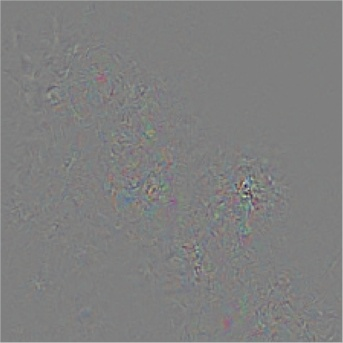
\includegraphics[width=0.13\linewidth]{figs/examples/googlenet/oxford/dog-cat4_diff_286} &
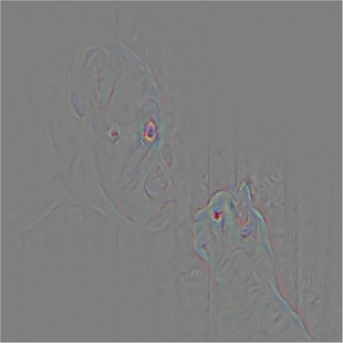
\includegraphics[width=0.13\linewidth]{figs/examples/googlenet/deconv/dog-cat4_diff_286} &
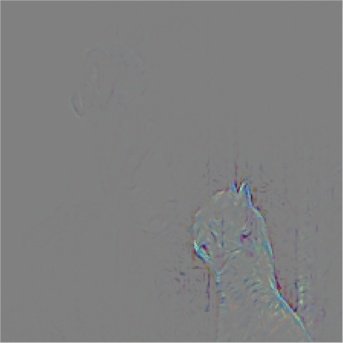
\includegraphics[width=0.13\linewidth]{figs/examples/googlenet/soft/dog-cat4_diff_286} \\
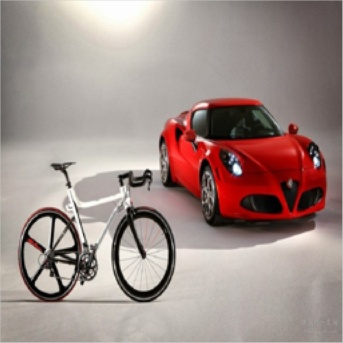
\includegraphics[width=0.13\linewidth]{figs/examples/googlenet/oxford/bic-car1} &
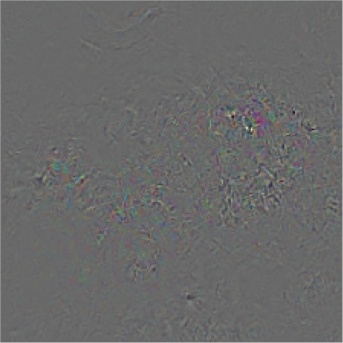
\includegraphics[width=0.13\linewidth]{figs/examples/googlenet/oxford/bic-car1_diff_818} &
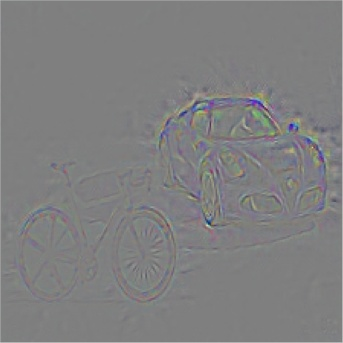
\includegraphics[width=0.13\linewidth]{figs/examples/googlenet/deconv/bic-car1_diff_818} &
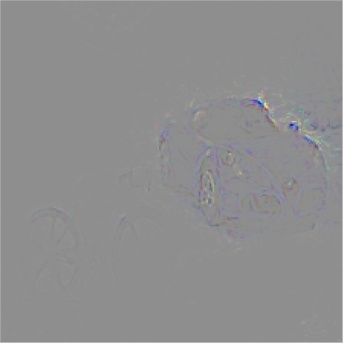
\includegraphics[width=0.13\linewidth]{figs/examples/googlenet/soft/bic-car1_diff_818} &
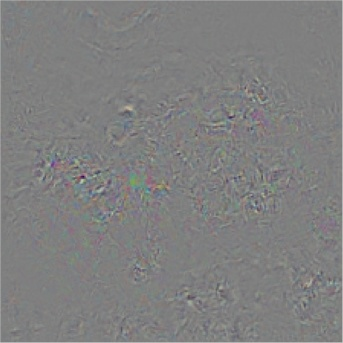
\includegraphics[width=0.13\linewidth]{figs/examples/googlenet/oxford/bic-car1_diff_672} &
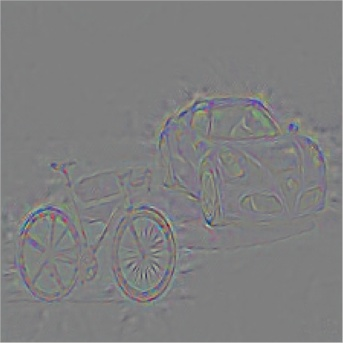
\includegraphics[width=0.13\linewidth]{figs/examples/googlenet/deconv/bic-car1_diff_672} &
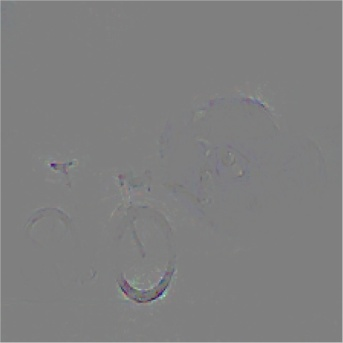
\includegraphics[width=0.13\linewidth]{figs/examples/googlenet/soft/bic-car1_diff_672} \\
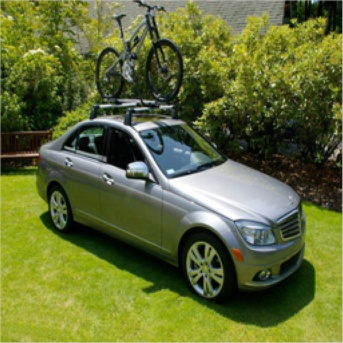
\includegraphics[width=0.13\linewidth]{figs/examples/googlenet/oxford/bic-car2} &
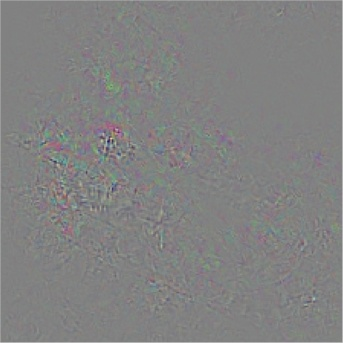
\includegraphics[width=0.13\linewidth]{figs/examples/googlenet/oxford/bic-car2_diff_818} &
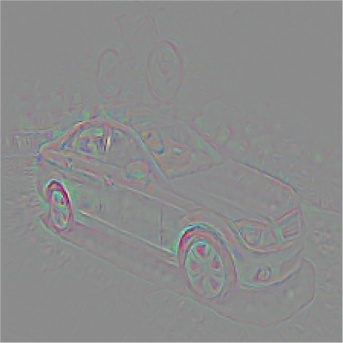
\includegraphics[width=0.13\linewidth]{figs/examples/googlenet/deconv/bic-car2_diff_818} &
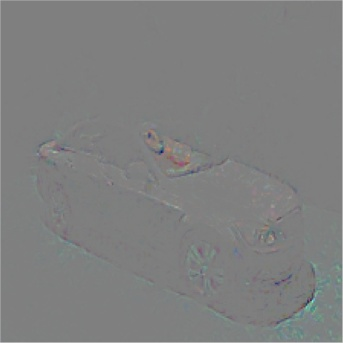
\includegraphics[width=0.13\linewidth]{figs/examples/googlenet/soft/bic-car2_diff_818} &
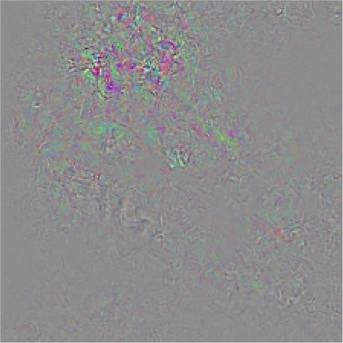
\includegraphics[width=0.13\linewidth]{figs/examples/googlenet/oxford/bic-car2_diff_672} &
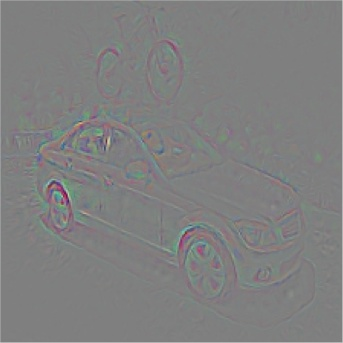
\includegraphics[width=0.13\linewidth]{figs/examples/googlenet/deconv/bic-car2_diff_672} &
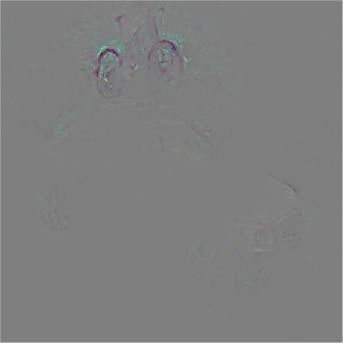
\includegraphics[width=0.13\linewidth]{figs/examples/googlenet/soft/bic-car2_diff_672} \\
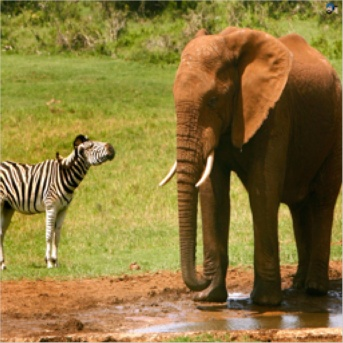
\includegraphics[width=0.13\linewidth]{figs/examples/googlenet/oxford/zeb-ele1} &
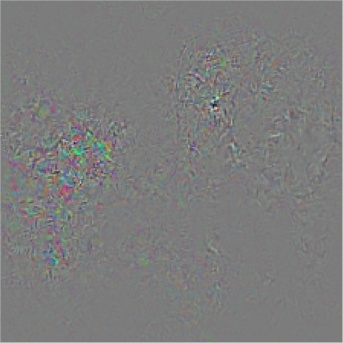
\includegraphics[width=0.13\linewidth]{figs/examples/googlenet/oxford/zeb-ele1_diff_341} &
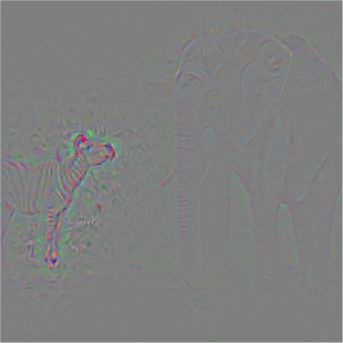
\includegraphics[width=0.13\linewidth]{figs/examples/googlenet/deconv/zeb-ele1_diff_341} &
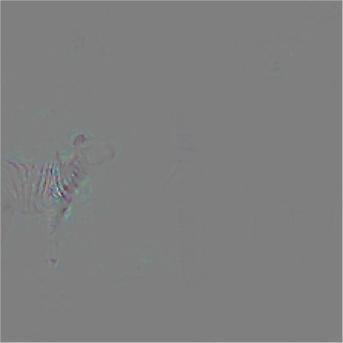
\includegraphics[width=0.13\linewidth]{figs/examples/googlenet/soft/zeb-ele1_diff_341} &
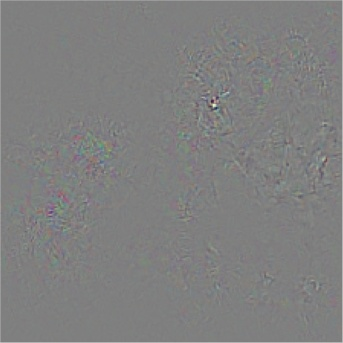
\includegraphics[width=0.13\linewidth]{figs/examples/googlenet/oxford/zeb-ele1_diff_387} &
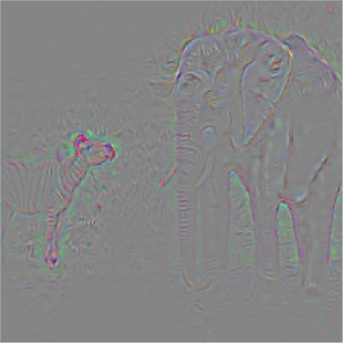
\includegraphics[width=0.13\linewidth]{figs/examples/googlenet/deconv/zeb-ele1_diff_387} &
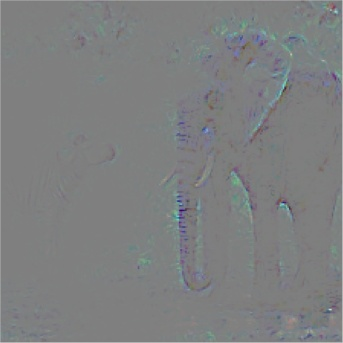
\includegraphics[width=0.13\linewidth]{figs/examples/googlenet/soft/zeb-ele1_diff_387} \\
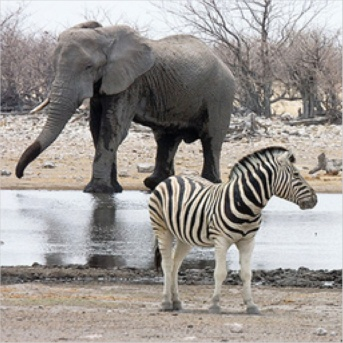
\includegraphics[width=0.13\linewidth]{figs/examples/googlenet/oxford/zeb-ele2} &
\includegraphics[width=0.13\linewidth]{figs/examples/googlenet/oxford/zeb-ele2_diff_341} &
\includegraphics[width=0.13\linewidth]{figs/examples/googlenet/deconv/zeb-ele2_diff_341} &
\includegraphics[width=0.13\linewidth]{figs/examples/googlenet/soft/zeb-ele2_diff_341} &
\includegraphics[width=0.13\linewidth]{figs/examples/googlenet/oxford/zeb-ele2_diff_387} &
\includegraphics[width=0.13\linewidth]{figs/examples/googlenet/deconv/zeb-ele2_diff_387} &
\includegraphics[width=0.13\linewidth]{figs/examples/googlenet/soft/zeb-ele2_diff_387} \\
{\small (a) Image} &
{\small (b) Gradient} &
{\small (c) Deconv} &
{\small (d) Feedback} &
{\small (e) Gradient} &
{\small (f) Deconv} &
{\small (g) Feedback} \\
& \multicolumn{3}{c||}{Object 1: dog, car, zebra} & \multicolumn{3}{|c}{Object 2: cat, bike, elephant} \\
\end{tabular}
% \vspace{-10pt}
\caption{We demonstrate the effectiveness of feedback neural networks for class-specific feature extraction, by comparing the class model visualization results against original gradient~\cite{simonyan2013deep} and Deconv~\cite{zeiler2014visualizing} on selected images with multiple objects. All methods compute visualizations on top a pre-trained GoogleNet. Column (a) shows the input images (\emph{i.e.} dog v.s. cat, car v.s. bike, and zebra v.s. elephant). Column (b) and (e) show the original image gradients. Column (c) and (f) show the deconv results. Column (d) and (g) show the image gradients after feedback. Comparing against original gradient and Deconv, the feedback visualization focus more on the correponding salient object area. Better viewed in color.} 
\label{fig:examples}
% \vspace{-30pt}
\end{center}
\end{figure*}


\begin{comment}
\setlength{\tabcolsep}{2pt}
\begin{figure*}
\begin{center}
\begin{tabular}{ccccccc}
\includegraphics[width=0.13\linewidth]{figs/examples/googlenet/soft/dog-cat1_sali_258} &
\includegraphics[width=0.13\linewidth]{figs/examples/googlenet/soft/dog-cat1_diff_258} &
\includegraphics[width=0.13\linewidth]{figs/examples/googlenet/oxford/dog-cat1_diff_258} &
\includegraphics[width=0.13\linewidth]{figs/examples/googlenet/oxford/dog-cat1} &
\includegraphics[width=0.13\linewidth]{figs/examples/googlenet/oxford/dog-cat1_diff_286} &
\includegraphics[width=0.13\linewidth]{figs/examples/googlenet/soft/dog-cat1_diff_286} &
\includegraphics[width=0.13\linewidth]{figs/examples/googlenet/soft/dog-cat1_sali_286} \\
\includegraphics[width=0.13\linewidth]{figs/examples/googlenet/soft/dog-cat2_sali_163} &
\includegraphics[width=0.13\linewidth]{figs/examples/googlenet/soft/dog-cat2_diff_163} &
\includegraphics[width=0.13\linewidth]{figs/examples/googlenet/oxford/dog-cat2_diff_163} &
\includegraphics[width=0.13\linewidth]{figs/examples/googlenet/oxford/dog-cat2} &
\includegraphics[width=0.13\linewidth]{figs/examples/googlenet/oxford/dog-cat2_diff_286} &
\includegraphics[width=0.13\linewidth]{figs/examples/googlenet/soft/dog-cat2_diff_286} &
\includegraphics[width=0.13\linewidth]{figs/examples/googlenet/soft/dog-cat2_sali_286} \\
\includegraphics[width=0.13\linewidth]{figs/examples/googlenet/soft/dog-cat3_sali_188} &
\includegraphics[width=0.13\linewidth]{figs/examples/googlenet/soft/dog-cat3_diff_188} &
\includegraphics[width=0.13\linewidth]{figs/examples/googlenet/oxford/dog-cat3_diff_188} &
\includegraphics[width=0.13\linewidth]{figs/examples/googlenet/oxford/dog-cat3} &
\includegraphics[width=0.13\linewidth]{figs/examples/googlenet/oxford/dog-cat3_diff_286} &
\includegraphics[width=0.13\linewidth]{figs/examples/googlenet/soft/dog-cat3_diff_286} &
\includegraphics[width=0.13\linewidth]{figs/examples/googlenet/soft/dog-cat3_sali_286} \\
\includegraphics[width=0.13\linewidth]{figs/examples/googlenet/soft/dog-cat4_sali_243} &
\includegraphics[width=0.13\linewidth]{figs/examples/googlenet/soft/dog-cat4_diff_243} &
\includegraphics[width=0.13\linewidth]{figs/examples/googlenet/oxford/dog-cat4_diff_243} &
\includegraphics[width=0.13\linewidth]{figs/examples/googlenet/oxford/dog-cat4} &
\includegraphics[width=0.13\linewidth]{figs/examples/googlenet/oxford/dog-cat4_diff_286} &
\includegraphics[width=0.13\linewidth]{figs/examples/googlenet/soft/dog-cat4_diff_286} &
\includegraphics[width=0.13\linewidth]{figs/examples/googlenet/soft/dog-cat4_sali_286} \\
\includegraphics[width=0.13\linewidth]{figs/examples/googlenet/soft/bic-car1_sali_818} &
\includegraphics[width=0.13\linewidth]{figs/examples/googlenet/soft/bic-car1_diff_818} &
\includegraphics[width=0.13\linewidth]{figs/examples/googlenet/oxford/bic-car1_diff_818} &
\includegraphics[width=0.13\linewidth]{figs/examples/googlenet/oxford/bic-car1} &
\includegraphics[width=0.13\linewidth]{figs/examples/googlenet/oxford/bic-car1_diff_672} &
\includegraphics[width=0.13\linewidth]{figs/examples/googlenet/soft/bic-car1_diff_672} &
\includegraphics[width=0.13\linewidth]{figs/examples/googlenet/soft/bic-car1_sali_672} \\
\includegraphics[width=0.13\linewidth]{figs/examples/googlenet/soft/bic-car2_sali_818} &
\includegraphics[width=0.13\linewidth]{figs/examples/googlenet/soft/bic-car2_diff_818} &
\includegraphics[width=0.13\linewidth]{figs/examples/googlenet/oxford/bic-car2_diff_818} &
\includegraphics[width=0.13\linewidth]{figs/examples/googlenet/oxford/bic-car2} &
\includegraphics[width=0.13\linewidth]{figs/examples/googlenet/oxford/bic-car2_diff_672} &
\includegraphics[width=0.13\linewidth]{figs/examples/googlenet/soft/bic-car2_diff_672} &
\includegraphics[width=0.13\linewidth]{figs/examples/googlenet/soft/bic-car2_sali_672} \\
\includegraphics[width=0.13\linewidth]{figs/examples/googlenet/soft/zeb-ele1_sali_341} &
\includegraphics[width=0.13\linewidth]{figs/examples/googlenet/soft/zeb-ele1_diff_341} &
\includegraphics[width=0.13\linewidth]{figs/examples/googlenet/oxford/zeb-ele1_diff_341} &
\includegraphics[width=0.13\linewidth]{figs/examples/googlenet/oxford/zeb-ele1} &
\includegraphics[width=0.13\linewidth]{figs/examples/googlenet/oxford/zeb-ele1_diff_387} &
\includegraphics[width=0.13\linewidth]{figs/examples/googlenet/soft/zeb-ele1_diff_387} &
\includegraphics[width=0.13\linewidth]{figs/examples/googlenet/soft/zeb-ele1_sali_387} \\
\includegraphics[width=0.13\linewidth]{figs/examples/googlenet/soft/zeb-ele2_sali_341} &
\includegraphics[width=0.13\linewidth]{figs/examples/googlenet/soft/zeb-ele2_diff_341} &
\includegraphics[width=0.13\linewidth]{figs/examples/googlenet/oxford/zeb-ele2_diff_341} &
\includegraphics[width=0.13\linewidth]{figs/examples/googlenet/oxford/zeb-ele2} &
\includegraphics[width=0.13\linewidth]{figs/examples/googlenet/oxford/zeb-ele2_diff_387} &
\includegraphics[width=0.13\linewidth]{figs/examples/googlenet/soft/zeb-ele2_diff_387} &
\includegraphics[width=0.13\linewidth]{figs/examples/googlenet/soft/zeb-ele2_sali_387} \\
{\small (a) Saliency} &
{\small (b) Feedback} &
{\small (c) Gradient} &
{\small (d) Image} &
{\small (e) Gradient} &
{\small (f) Feedback} &
{\small (g) Saliency}
\end{tabular}
% \vspace{-10pt}
\caption{We illustrate the effectiveness of feedback neural networks (built on a pre-trained GoogleNet) for class-specific feature extraction. Column (d) shows the selected input images containing two different objects (i.e.\ dog v.s. cat, car v.s. bike, and zebra v.s. elephant). Column (c) and (e) show the orignal image gradients of the two different classes. Column (b) and (f) show the image gradients after feedback net finishes adjusting hidden neuron activiations w.r.t. the two different classes. Column (a) and (g) show the salience map computed from the gradients after feedback. Comparing against the orignal image gradients in (c) and (e) which usually spread over the entire image, feedbacked gradients in (b) and (f) focus more on the corresponding object area. Better viewed in color.}
\label{fig:examples}
% \vspace{-30pt}
\end{center}
\end{figure*}
\end{comment}

\setlength{\tabcolsep}{2pt}
\begin{figure*}
\begin{center}
\begin{tabular}{cccccccc}
\rotatebox{90}{\hspace{5mm}Gradient} &
\includegraphics[width=0.13\linewidth]{figs/examples/alexnet/soft/zeb-ele1_diff_341} &
\includegraphics[width=0.13\linewidth]{figs/examples/vggnet/soft/zeb-ele1_diff_341} &
\includegraphics[width=0.13\linewidth]{figs/examples/googlenet/soft/zeb-ele1_diff_341} &
\includegraphics[width=0.13\linewidth]{figs/examples/googlenet/soft/zeb-ele1} &
\includegraphics[width=0.13\linewidth]{figs/examples/alexnet/soft/zeb-ele1_diff_387} &
\includegraphics[width=0.13\linewidth]{figs/examples/vggnet/soft/zeb-ele1_diff_387} &
\includegraphics[width=0.13\linewidth]{figs/examples/googlenet/soft/zeb-ele1_diff_387} \\
\rotatebox{90}{\hspace{5mm}Saliency} &
\includegraphics[width=0.13\linewidth]{figs/examples/alexnet/soft/zeb-ele1_sali_341} &
\includegraphics[width=0.13\linewidth]{figs/examples/vggnet/soft/zeb-ele1_sali_341} &
\includegraphics[width=0.13\linewidth]{figs/examples/googlenet/soft/zeb-ele1_sali_341} &
\includegraphics[width=0.13\linewidth]{figs/examples/googlenet/soft/zeb-ele1} &
\includegraphics[width=0.13\linewidth]{figs/examples/alexnet/soft/zeb-ele1_sali_387} &
\includegraphics[width=0.13\linewidth]{figs/examples/vggnet/soft/zeb-ele1_sali_387} &
\includegraphics[width=0.13\linewidth]{figs/examples/googlenet/soft/zeb-ele1_sali_387} \\
\rotatebox{90}{\hspace{5mm}Gradient} &
\includegraphics[width=0.13\linewidth]{figs/examples/alexnet/soft/zeb-ele2_diff_341} &
\includegraphics[width=0.13\linewidth]{figs/examples/vggnet/soft/zeb-ele2_diff_341} &
\includegraphics[width=0.13\linewidth]{figs/examples/googlenet/soft/zeb-ele2_diff_341} &
\includegraphics[width=0.13\linewidth]{figs/examples/googlenet/soft/zeb-ele2} &
\includegraphics[width=0.13\linewidth]{figs/examples/alexnet/soft/zeb-ele2_diff_387} &
\includegraphics[width=0.13\linewidth]{figs/examples/vggnet/soft/zeb-ele2_diff_387} &
\includegraphics[width=0.13\linewidth]{figs/examples/googlenet/soft/zeb-ele2_diff_387} \\
\rotatebox{90}{\hspace{5mm}Saliency} &
\includegraphics[width=0.13\linewidth]{figs/examples/alexnet/soft/zeb-ele2_sali_341} &
\includegraphics[width=0.13\linewidth]{figs/examples/vggnet/soft/zeb-ele2_sali_341} &
\includegraphics[width=0.13\linewidth]{figs/examples/googlenet/soft/zeb-ele2_sali_341} &
\includegraphics[width=0.13\linewidth]{figs/examples/googlenet/soft/zeb-ele2} &
\includegraphics[width=0.13\linewidth]{figs/examples/alexnet/soft/zeb-ele2_sali_387} &
\includegraphics[width=0.13\linewidth]{figs/examples/vggnet/soft/zeb-ele2_sali_387} &
\includegraphics[width=0.13\linewidth]{figs/examples/googlenet/soft/zeb-ele2_sali_387} \\
\rotatebox{90}{\hspace{5mm}Gradient} &
\includegraphics[width=0.13\linewidth]{figs/examples/alexnet/soft/bic-car1_diff_818} &
\includegraphics[width=0.13\linewidth]{figs/examples/vggnet/soft/bic-car1_diff_818} &
\includegraphics[width=0.13\linewidth]{figs/examples/googlenet/soft/bic-car1_diff_818} &
\includegraphics[width=0.13\linewidth]{figs/examples/googlenet/soft/bic-car1} &
\includegraphics[width=0.13\linewidth]{figs/examples/alexnet/soft/bic-car1_diff_672} &
\includegraphics[width=0.13\linewidth]{figs/examples/vggnet/soft/bic-car1_diff_672} &
\includegraphics[width=0.13\linewidth]{figs/examples/googlenet/soft/bic-car1_diff_672} \\
\rotatebox{90}{\hspace{5mm}Saliency} &
\includegraphics[width=0.13\linewidth]{figs/examples/alexnet/soft/bic-car1_sali_818} &
\includegraphics[width=0.13\linewidth]{figs/examples/vggnet/soft/bic-car1_sali_818} &
\includegraphics[width=0.13\linewidth]{figs/examples/googlenet/soft/bic-car1_sali_818} &
\includegraphics[width=0.13\linewidth]{figs/examples/googlenet/soft/bic-car1} &
\includegraphics[width=0.13\linewidth]{figs/examples/alexnet/soft/bic-car1_sali_672} &
\includegraphics[width=0.13\linewidth]{figs/examples/vggnet/soft/bic-car1_sali_672} &
\includegraphics[width=0.13\linewidth]{figs/examples/googlenet/soft/bic-car1_sali_672} \\
\rotatebox{90}{\hspace{5mm}Gradient} &
\includegraphics[width=0.13\linewidth]{figs/examples/alexnet/soft/bic-car2_diff_818} &
\includegraphics[width=0.13\linewidth]{figs/examples/vggnet/soft/bic-car2_diff_818} &
\includegraphics[width=0.13\linewidth]{figs/examples/googlenet/soft/bic-car2_diff_818} &
\includegraphics[width=0.13\linewidth]{figs/examples/googlenet/soft/bic-car2} &
\includegraphics[width=0.13\linewidth]{figs/examples/alexnet/soft/bic-car2_diff_672} &
\includegraphics[width=0.13\linewidth]{figs/examples/vggnet/soft/bic-car2_diff_672} &
\includegraphics[width=0.13\linewidth]{figs/examples/googlenet/soft/bic-car2_diff_672} \\
\rotatebox{90}{\hspace{5mm}Saliency} &
\includegraphics[width=0.13\linewidth]{figs/examples/alexnet/soft/bic-car2_sali_818} &
\includegraphics[width=0.13\linewidth]{figs/examples/vggnet/soft/bic-car2_sali_818} &
\includegraphics[width=0.13\linewidth]{figs/examples/googlenet/soft/bic-car2_sali_818} &
\includegraphics[width=0.13\linewidth]{figs/examples/googlenet/soft/bic-car2} &
\includegraphics[width=0.13\linewidth]{figs/examples/alexnet/soft/bic-car2_sali_672} &
\includegraphics[width=0.13\linewidth]{figs/examples/vggnet/soft/bic-car2_sali_672} &
\includegraphics[width=0.13\linewidth]{figs/examples/googlenet/soft/bic-car2_sali_672} \\
&
{\small (a) AlexNet} &
{\small (b) VggNet} &
{\small (c) GoogleNet} &
{\small (d) Image} &
{\small (e) AlexNet} &
{\small (f) VggNet} &
{\small (g) GoogleNet}
\end{tabular}
% \vspace{-10pt}
\caption{We visualize the feedback ability of three most popular pre-trained ConvNets: AlexNet, VggNet and GoogleNet. We show the input images in column (d). We show the feedbacked image gradients and salience maps for each image. On the left 3 columns, we compute the results w.r.t. zebra or car, on the right 3 columns we compute the results w.r.t. elephant or bike. In the visualization results, VggNet performs quite better than AlexNet, especially in capturing the most salient object details, suggesting the benefit of usage of small convolutional filters and deeper structures. Although both VggNet and GogoleNet produce similar classification accruacy, we find GoogleNet provides the better class specific feature separations. We suspect the two 4096 fully connected layers in VggNet (which GoogleNetdoes not have) could harm the spatial distinctiveness of image features.}
\label{fig:model_compare}
% \vspace{-30pt}
\end{center}
\end{figure*}

\setlength{\tabcolsep}{2pt}
\begin{figure*}
\begin{center}
\begin{tabular}{ccccccc}
{\small (a) Image} &
{\small (b) G. pyrenees} &
{\small (c) Beagle} &
{\small (d) York. terrier} &
{\small (e) Kit fox} &
{\small (f) Tiger} &
{\small (g) Ostrich} \\
&
\includegraphics[width=0.13\linewidth]{figs/class_compare/pyrenees} &
\includegraphics[width=0.13\linewidth]{figs/class_compare/beagle} &
\includegraphics[width=0.13\linewidth]{figs/class_compare/yorkshire-terrier} &
\includegraphics[width=0.13\linewidth]{figs/class_compare/kit-fox} &
\includegraphics[width=0.13\linewidth]{figs/class_compare/tiger} &
\includegraphics[width=0.13\linewidth]{figs/class_compare/ostrich} \\
\includegraphics[width=0.13\linewidth]{figs/class_compare/googlenet/soft/dog-cat1} &
\includegraphics[width=0.13\linewidth]{figs/class_compare/googlenet/soft/dog-cat1_diff_258} &
\includegraphics[width=0.13\linewidth]{figs/class_compare/googlenet/soft/dog-cat1_diff_163} &
\includegraphics[width=0.13\linewidth]{figs/class_compare/googlenet/soft/dog-cat1_diff_188} &
\includegraphics[width=0.13\linewidth]{figs/class_compare/googlenet/soft/dog-cat1_diff_279} &
\includegraphics[width=0.13\linewidth]{figs/class_compare/googlenet/soft/dog-cat1_diff_293} &
\includegraphics[width=0.13\linewidth]{figs/class_compare/googlenet/soft/dog-cat1_diff_10} \\
\includegraphics[width=0.13\linewidth]{figs/class_compare/googlenet/soft/dog-cat2} &
\includegraphics[width=0.13\linewidth]{figs/class_compare/googlenet/soft/dog-cat2_diff_258} &
\includegraphics[width=0.13\linewidth]{figs/class_compare/googlenet/soft/dog-cat2_diff_163} &
\includegraphics[width=0.13\linewidth]{figs/class_compare/googlenet/soft/dog-cat2_diff_188} &
\includegraphics[width=0.13\linewidth]{figs/class_compare/googlenet/soft/dog-cat2_diff_279} &
\includegraphics[width=0.13\linewidth]{figs/class_compare/googlenet/soft/dog-cat2_diff_293} &
\includegraphics[width=0.13\linewidth]{figs/class_compare/googlenet/soft/dog-cat2_diff_10} \\
\includegraphics[width=0.13\linewidth]{figs/class_compare/googlenet/soft/dog-cat3} &
\includegraphics[width=0.13\linewidth]{figs/class_compare/googlenet/soft/dog-cat3_diff_258} &
\includegraphics[width=0.13\linewidth]{figs/class_compare/googlenet/soft/dog-cat3_diff_163} &
\includegraphics[width=0.13\linewidth]{figs/class_compare/googlenet/soft/dog-cat3_diff_188} &
\includegraphics[width=0.13\linewidth]{figs/class_compare/googlenet/soft/dog-cat3_diff_279} &
\includegraphics[width=0.13\linewidth]{figs/class_compare/googlenet/soft/dog-cat3_diff_293} &
\includegraphics[width=0.13\linewidth]{figs/class_compare/googlenet/soft/dog-cat3_diff_10} \\
\end{tabular}
% \vspace{-10pt}
\caption{We show some interesting visualizations for the understanding of fine-grained classification by comparsing against the feedback gradients of ground truth labels and other classes. The top row shows the class labels and a representative image for each class for the ease of understanding. Column (a) shows the three examplar input images, their ground truth labels are great pyrenees, beagle and yorkshire terrier respectively. We can see that although (b), (c) and (d) are all dogs, their salient area for distinction are quite different. Noses are one of the most important feature for classifying dogs, but ears are specific feature for beagles, while fluffy is more importatnt to yorkshire terrier. When the top down is from (e) kit fox, features on the cat in the last row is more fox-specific: nose and ears. When top down is from (f) tiger, features on the same at is more tiger-specific: textures. And when it's (g) ostrich, nothing special come out.}
\label{fig:class_compare}
% \vspace{-30pt}
\end{center}
\end{figure*}
